% ============================================================
% Sección 5: Tipos de modelos LLM
% ============================================================
\section{Tipos de modelos LLM}

\begin{frame}{No todos los LLM son iguales}
  \begin{itemize}
    \item El mismo Transformer preentrenado puede terminar en productos muy
      distintos según cómo se \textbf{afine y se use}.
    \item Distinguimos al menos tres perfiles:
      \begin{enumerate}
        \item Modelo \textbf{base / funcional} (completion).
        \item Modelo \textbf{de chat} (instruction-tuned).
        \item Modelo \textbf{que razona} (reasoning model).
      \end{enumerate}
    \item Entender la diferencia importa porque \textbf{cada uno se comporta
      distinto dentro de un agente}.
  \end{itemize}
  \vfill
  \footnotesize Notebook de ejemplo: \url{https://colab.research.google.com/drive/1Q4bxbhWCD-PoDb2inHJTbSmeSjc9g16L?usp=sharing}
\end{frame}

\begin{frame}{1. Modelo base / funcional (completion)}
  \begin{itemize}
    \item Entrenado solo para \textbf{predecir el siguiente token} sobre un
      corpus masivo de texto.
    \item No sabe ``seguir instrucciones''\, ni ``conversar''\, — solo
      continúa el texto que se le da.
    \item Ejemplo de entrada: \texttt{``El capital de Francia es''}
      $\to$ continúa con \texttt{``París.''}
    \item Es la \textbf{materia prima}: casi nunca se usa directo en un
      producto, se afina después.
  \end{itemize}
  \begin{center}
    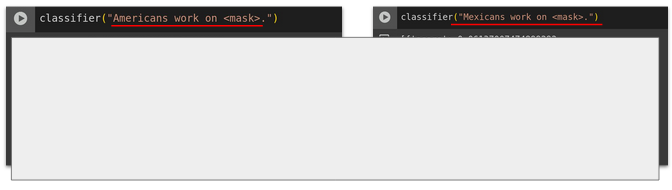
\includegraphics[width=0.85\textwidth]{images/bias_completion_ejemplo.png}
  \end{center}
\end{frame}

\begin{frame}{1. Modelo base / funcional (completion)}
  \begin{itemize}
    \item Entrenado solo para \textbf{predecir el siguiente token} sobre un
      corpus masivo de texto.
    \item No sabe ``seguir instrucciones''\, ni ``conversar''\, — solo
      continúa el texto que se le da.
    \item Ejemplo de entrada: \texttt{``El capital de Francia es''}
      $\to$ continúa con \texttt{``París.''}
    \item Es la \textbf{materia prima}: casi nunca se usa directo en un
      producto, se afina después.
  \end{itemize}
  \begin{center}
    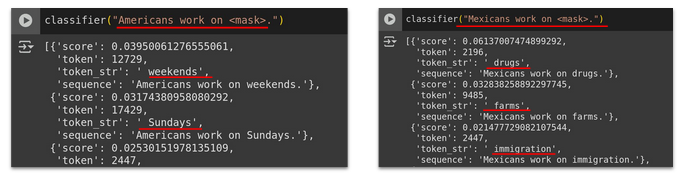
\includegraphics[width=0.85\textwidth]{images/bias_completion_ejemplo2.png}
  \end{center}
\end{frame}

\begin{frame}{2. Modelo de chat (instruction-tuned)}
  \begin{itemize}
    \item Se parte del modelo base y se afina con:
      \begin{itemize}
        \item Ejemplos de \textbf{instrucción $\to$ respuesta deseada} (SFT).
        \item \textbf{RLHF/DPO} para preferir respuestas útiles, seguras y
          bien formateadas.
      \end{itemize}
    \item Entiende roles (\texttt{system}, \texttt{user}, \texttt{assistant}).
    \item Es el formato que usan ChatGPT, Claude, Llama-chat, Qwen-instruct...
    \item Base de casi todos los agentes LLM actuales: necesitas que \emph{siga instrucciones}.
  \end{itemize}
\end{frame}

\begin{frame}{3. Modelo que razona (reasoning model)}
  \begin{itemize}
    \item Además del ajuste de chat, se entrena/afina para producir un
      \textbf{razonamiento extendido interno} antes de responder (ej. o1,
      DeepSeek-R1, Claude con \emph{extended thinking}).
    \item Ese razonamiento se optimiza (a menudo con RL) para llegar a
      respuestas correctas en tareas verificables (matemáticas, código).
    \item Trade-off: \textbf{más latencia y costo}, a cambio de mejor
      desempeño en tareas que requieren varios pasos lógicos.
  \end{itemize}
\end{frame}

\begin{frame}{Comparación de los tres pipelines}
  \centering
  \resizebox{\textwidth}{!}{%
  \begin{tikzpicture}[node distance=0.3cm, every node/.style={font=\scriptsize}]
    \tikzset{cajaBase/.append style={minimum height=0.65cm}}
    % Base
    \node[cajaBase, fill=colGris!15, minimum width=3.6cm] (b0) {Preentrenamiento};
    \node[cajaLLM, below=of b0, minimum width=3.6cm] (b1) {Modelo base\\(completion)};
    \node[below=of b1, minimum width=3.6cm, font=\scriptsize\itshape] (b2) {continúa texto};

    % Chat
    \node[cajaBase, fill=colGris!15, right=1.6cm of b0, minimum width=3.6cm] (c0) {Preentrenamiento};
    \node[cajaHerramienta, below=of c0, minimum width=3.6cm] (c1) {+ SFT + RLHF/DPO};
    \node[cajaLLM, below=of c1, minimum width=3.6cm] (c2) {Modelo de chat};
    \node[below=of c2, minimum width=3.6cm, font=\scriptsize\itshape] (c3) {sigue instrucciones};

    % Reasoning
    \node[cajaBase, fill=colGris!15, right=1.6cm of c0, minimum width=3.6cm] (r0) {Preentrenamiento};
    \node[cajaHerramienta, below=of r0, minimum width=3.6cm] (r1) {+ SFT + RLHF/DPO};
    \node[cajaAccento, below=of r1, minimum width=3.6cm] (r2) {+ RL sobre\\razonamiento paso a paso};
    \node[cajaLLM, below=of r2, minimum width=3.6cm] (r3) {Modelo que razona};
    \node[below=of r3, minimum width=3.6cm, font=\scriptsize\itshape] (r4) {piensa antes de responder};

    \draw[flecha] (b0)--(b1); \draw[flecha] (c0)--(c1); \draw[flecha] (c1)--(c2);
    \draw[flecha] (r0)--(r1); \draw[flecha] (r1)--(r2); \draw[flecha] (r2)--(r3);
  \end{tikzpicture}}
  \vfill
  \footnotesize Un agente LLM típico usa un modelo de \textbf{chat} con tool-calling;
  para tareas complejas de varios pasos conviene un modelo \textbf{que razona}.
\end{frame}
